\section{Computational Experiments}

Based on the above descriptios, we validated the performance of ACO on benchmark instances.
The algorithm was implemented in C++ on a Windows XP machine with Pentium IV 2.20GHz and 2G memory. 
Inasmuch as parameter settings have big impacts of ACO's efficiency, we identified the parameters using multiple trails and the final paramters are set as follows: the number of ants ($N\_ANT\_COUNT$) = number of tasks ($N\_TASK\_COUNT$), the maximum number of iterataions $N_{C_{max}} = 50$, $\tau_0 = 1$, $\alpha = 1.0$, $\beta = 2.0$, $\rho_1 = 0.1$, $\rho_2(t_0) = 1$, $\rho_{2_{min}} = 0.5$, $r_1 = 0.6$, $r_2 = 0.3$, $r_3 = 0.1$.

We first analyze the proposed ACO's performance based on the results for problem $C = 57$ from Kilbridge benchmark set, then present the overall performance comparison for all 24 benchmark problems in the set.
The task precedence graph and computational results for problem Kilbridge are given in Figure \ref{fig:fig1} and Table \ref{tab:tab1}, respectively.

\begin{figure}[h!]
	\begin{center}
		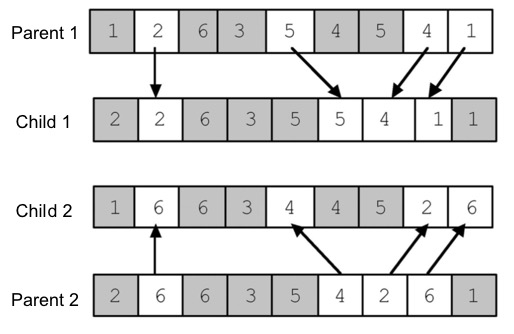
\includegraphics[width=0.6\linewidth]{sections/figure1.jpg}
		\caption{Task Precedence Graph of Problem Kilbridge}
		\label{fig:fig1}
	\end{center}
\end{figure}

\begin{table}[h!]
	\begin{center}
		\caption{Computational Result of Problem Kilbridge}
		\label{tab:tab1}
		\begin{tabular}{l|c|c|c}
			\hline
			\textbf{Workstation No.} & \textbf{Tasks} & \textbf{Workstation Time(s)} & \textbf{Free Time (s)}\\
			\hline
			1 & 1, 11, 12, 13, 15, 18, 39 & 55 & 2\\
			\hline
			2 & 2, 7, 8, 16 & 54 & 3\\
			\hline
			3 & 14, 17, 19, 20, 27, 31 & 57 & 0\\
			\hline
			4 & 21 & 55 & 2 \\
			\hline
			5 & 23, 24 & 56 & 1 \\
			\hline
			6 & 3, 4, 22, 30, 33, 34 & 57 & 0 \\
			\hline
			7 & 5, 25, 29, 36 & 56 & 1\\
			\hline
			8 & 6, 26, 28, 35 & 54 & 3 \\
			\hline
			9 & 9, 10, 32, 38, 40 & 55 & 2\\
			\hline
			10 & 37, 41, 42, 43, 44, 45 & 53 & 4\\
			\hline
		\end{tabular}
	\end{center}
\end{table}

It can be seen from the computational results that our proposed algorithm was able to identify the solution with minimal number of workstations and balance rate of 96.8\% for the problem Kilbridge.
Figure \ref{fig:fig2} shows the workstation workload is well balanced and the solution was identified within 1s, which proved the efficiency of the proposed algorithm.



\begin{figure}[h!]
	\begin{center}
		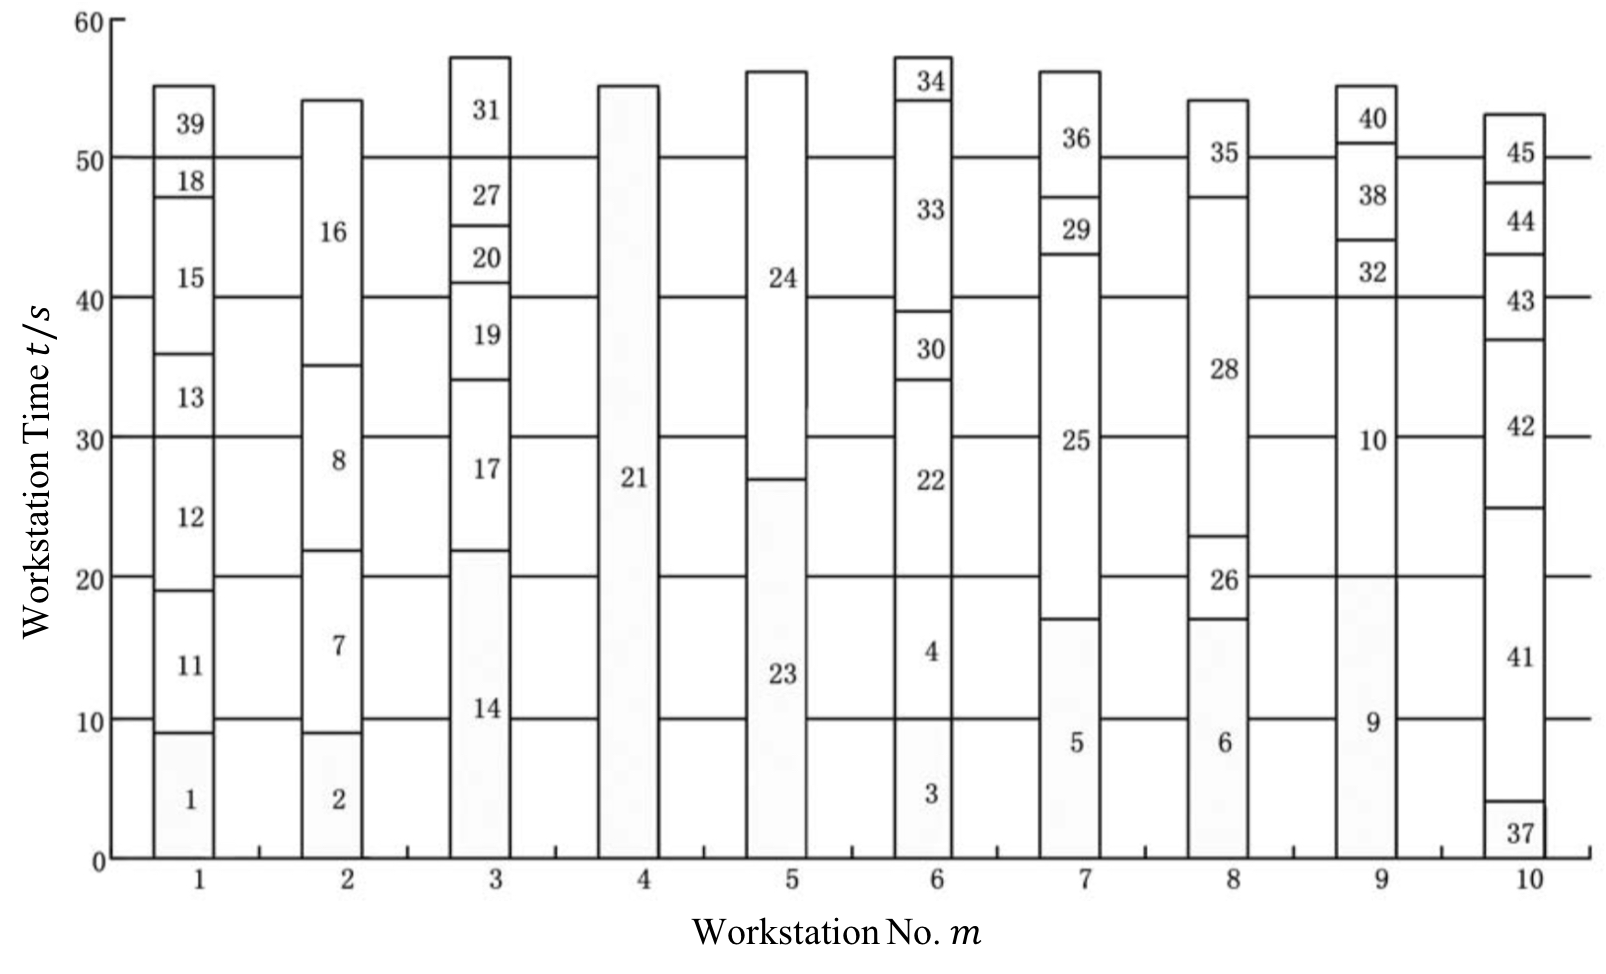
\includegraphics[width=0.8\linewidth]{sections/figure2.png}
		\caption{Task Precedence Graph of Problem Kilbridge}
		\label{fig:fig2}
	\end{center}
\end{figure}


Table \ref{tab:tab2} shows the computational results of the proposed algorithm with weighted algorithm and genetic algorithm (GA).
It can be seen from the table that both the proposed ACO and GA can identify the solution with minimal number of workstations for all the 24 benchmarking problems and their overall performance is superior than the weighted algorithm.
It is worth noting that the weighted algorithm uses a static precendence rule and its selection criterion is unique and deterministic; the proposed algorithm is stochastic in nature and it can fully utilize the information between ants and previous experience, which helps the algorithm jump out of local optima and therefore find the optimal solutions.



\begin{table}[h!]
	\label{tab:tab2}
	\centering
	\caption{Computational Result Comparisons on Benchmarking Problems}
	\resizebox{0.9\columnwidth}{!}{
	\begin{tabular}{c|c|c|c|c|c|c|c|c|c}
		\hline
		\multirow{2}{*}{Problem} & \multirow{2}{*}{No. Tasks $n$} & \multirow{2}{*}{Cycle $C$} & \multirow{2}{*}{Time $t_{sum}$} & \multirow{2}{*}{Min. No. Workstation $m_{min}$} & \multicolumn{3}{c|}{Adaptive ACO} & \multirow{2}{*}{Weight} & \multirow{2}{*}{GA} \\
		\cline{6-8}
		& & & & & m & L & I & & \\
		\hline
		\multirow{2}{*}{Jackson} & \multirow{2}{*}{11} & 10 & \multirow{2}{*}{46} & 5 & 5 & 92.0\% & 1.095 & 6 & 5\\
		\cline{3-3}
		\cline{5-10}
		& & 13 & & 4& 4& 88.5\% & 0.707 &4 & 4\\
		\hline
		\multirow{2}{*}{Heskiaoff} & \multirow{2}{*}{28} & 205 & \multirow{2}{*}{1024} & 5 & 5 & 99.9\% & 0.447 & 6 & 5\\
		\cline{3-3}
		\cline{5-10}
		& & 256 & & 4& 4& 100.0\% & 0 &5 & 4\\
		\hline
		\multirow{3}{*}{Buxey} & \multirow{3}{*}{29} & 30 & \multirow{3}{*}{324} & 12 & 12 & 90.0\% & 2.309 & 12 & 12\\
		\cline{3-3}
		\cline{5-10}
		& & 41 & & 8& 8& 98.8\% & 0.707 &9 & 8\\
		\cline{3-3}
		\cline{5-10}
		& & 54 & & 7& 7& 85.7\% & 4.629 &7 & 7\\
		\hline
		\multirow{2}{*}{Sawyer} & \multirow{2}{*}{30} & 41 & \multirow{2}{*}{324} & 8 & 8 & 98.8\% & 0.707 & 9 & 8\\
		\cline{3-3}
		\cline{5-10}
		& & 47 & & 7& 7& 98.5\% & 2.390 &8 & 7\\
		\hline
		\multirow{4}{*}{Lutzl} & \multirow{4}{*}{32} & 1414 & \multirow{4}{*}{14140} & 11 & 11 & 90.9\% & 134.400 & 12 & 11\\
		\cline{3-3}
		\cline{5-10}
		& & 1572 & & 10& 10& 89.9\% & 134.270 &11 & 10\\
		\cline{3-3}
		\cline{5-10}
		& & 2020 & & 8& 8& 87.5\% & 110.640 &8 & 8\\
		\cline{3-3}
		\cline{5-10}
		& & 2828 & & 6& 6& 83.3\% & 449.620 &6 & 6\\
		\hline
		\multirow{6}{*}{Kilbridge} & \multirow{6}{*}{45} & 57 & \multirow{6}{*}{552} & 10 & 10 & 96.8\% & 2.240 & 11 & 10\\
		\cline{3-3}
		\cline{5-10}
		& & 79 & & 7& 7& 99.8\% & 0.377 &8 & 7\\
		\cline{3-3}
		\cline{5-10}
		& & 92 & & 6& 6& 100.0\% & 0 &7 & 6\\
		\cline{3-3}
		\cline{5-10}
		& & 110 & & 6& 6& 83.6\% & 18.876 &6 & 6\\
		\cline{3-3}
		\cline{5-10}
		& & 138 & & 4& 4& 100.0\% & 0 &5 & 4\\
		\cline{3-3}
		\cline{5-10}
		& & 184 & & 3& 3& 100.0\% & 0 &4 & 3\\
		\hline
		\multirow{5}{*}{Tonge} & \multirow{5}{*}{70} & 176 & \multirow{5}{*}{3510} & 21 & 21 & 95.0\% & 8.423 & 22 & 21\\
		\cline{3-3}
		\cline{5-10}
		& & 364 & & 10& 10& 96.4\% & 4.795 &11 & 10\\
		\cline{3-3}
		\cline{5-10}
		& & 410 & & 9& 9& 95.1\% & 6.896 &10 & 9\\
		\cline{3-3}
		\cline{5-10}
		& & 468 & & 8& 8& 93.8\% & 15.050 &8 & 8\\
		\cline{3-3}
		\cline{5-10}
		& & 527 & & 7& 7& 95.1\% & 14.540 &7 & 7\\
		\hline
	\end{tabular}}
	
\end{table}